\chapter{Mathematical Foundations and Safety Guarantees}
\label{ch:mathematical-foundations}

\section{Why the theorem surface is promotion-gated}
ORIUS is not defended by one grand theorem claiming safety for every plant,
every sensor regime, and every domain.  The mathematical surface is defended by
a promotion gate: every active theorem-like row must have a statement,
assumptions, proof, code anchor, tests, artifact evidence, artifact hashes, and
a claim-boundary note before it is allowed to appear as a flagship theorem,
flagship corollary, flagship lemma, or flagship definition.

The current manuscript-facing truth source is the theorem promotion matrix in
\path{reports/publication/theorem_promotion_matrix.csv} and the corresponding
result cards in \path{reports/publication/theorem_result_cards/}.  Historical
draft/proxy rows are retained only as archived audit context; they are not part
of the defended theorem register.  This keeps the dissertation from making a
false choice between abstraction and implementation.  The theorem surface is
written against typed runtime objects, explicit assumptions, and
artifact-backed diagnostics.  As a result, the strongest claims are not merely
conceptual and they are not merely empirical.

\section{Notation and assumption discipline}
The formal objects used in this chapter are simple but exact:
\begin{itemize}
  \item a latent physical state $x_t$;
  \item an observed state or telemetry-derived state $z_t$;
  \item a candidate action $a_t$ proposed by nominal intelligence;
  \item a repaired or fallback action $\tilde{a}_t$ released by ORIUS;
  \item a runtime reliability score $w_t \in [0,1]$ summarizing observation trust; and
  \item a violation predicate $\mathcal{V}(x_t, a_t)$ defined through the domain adapter.
\end{itemize}

The score $w_t$ is not interpreted as a probability by definition. Whenever a
theorem turns $w_t$ into a probabilistic risk or indistinguishability claim,
that conversion is written as an extra theorem-local assumption.

The dissertation does not hide its assumptions. Every strong statement depends on the
assumption register in Appendix~\ref{app:assumptions}. The core assumptions are finite
observation-consistent state inflation, availability of a feasible repaired action or
bounded fallback, causal certificate issuance, dual-trajectory replay fidelity, adapter
faithfulness, and evidence-tier discipline. If any of those assumptions is violated, the
associated theorem is not silently inherited by the runtime row.

\section{Definition of OASG as a formal event}
\begin{definition}[Observation--Action Safety Gap]
An observation--action safety gap occurs at time $t$ when the candidate action is admissible
under the observed state but unsafe under the true physical state:
\[
\mathcal{S}_{\mathrm{obs}}(z_t, a_t)=1 \quad \text{and} \quad \mathcal{V}(x_t, a_t)=1.
\]
\end{definition}

This definition is deliberately agnostic to plant family. The adapter chooses the local
meaning of admissibility and true-state violation. The universal layer fixes the semantic
pattern of the failure event.

\section{The paper-facing theorem surface}
The paper-facing theory chapter now carries a flagship-grade theorem package,
not merely a short narrative subset.  The permanent T1--T11 labels remain
stable for traceability, while newer scoped surfaces use stable identifiers such
as \texttt{T11\_Byzantine}, \texttt{T\_stale\_decay},
\texttt{T\_minimax}, and \texttt{T\_sensor\_converse}.  The claim is
deliberately conditional: ORIUS is safety-optimal under covered observation
ambiguity, not globally optimal for every possible physical-AI system.

\begin{table}[htbp]
\centering
\scriptsize
\caption{Promotion-gated theorem package synchronized with the repository result cards.}
\label{tab:promotion-gated-theorem-package}
\resizebox{\linewidth}{!}{%
\begin{tabular}{llll}
\toprule
\textbf{Surface} & \textbf{Promoted status} & \textbf{Defended claim boundary} & \textbf{Result-card evidence}\\
\midrule
T1--T4 & Flagship theorems / corollaries & OASG, one-step preservation, envelope, and observation necessity under stated assumptions & \path{reports/publication/theorem_result_cards/T1.json}--\path{T4.json}\\
T5 & Flagship theorem & Finite-horizon certificate validity; invalidates on contradictory evidence & \path{reports/publication/theorem_result_cards/T5.json}\\
T6--T8 & Flagship theorems & Expiration, feasible fallback, and graceful degradation with useful work & \path{reports/publication/theorem_result_cards/T6.json}--\path{T8.json}\\
T9--T10 & Flagship theorems & Mandatory-release impossibility and two-state boundary lower bound & \path{reports/publication/theorem_result_cards/T9.json}--\path{T10.json}\\
\texttt{T10\_T11} sandwich & Flagship corollary & Observation-only lower bound versus ORIUS $\alpha$-covered upper bound & \path{reports/publication/theorem_result_cards/T10_T11_ObservationAmbiguitySandwich.json}\\
T11 and domain lemmas & Flagship theorem / lemmas & Typed structural transfer and bounded AV/Healthcare runtime postconditions & \path{reports/publication/theorem_result_cards/T11.json}\\
\texttt{T11\_Byzantine} & Flagship theorem & Robust aggregation only for $b<n/2$ Byzantine channels & \path{reports/publication/theorem_result_cards/T11_Byzantine.json}\\
\texttt{T\_stale\_decay} & Flagship theorem & Stale-hold uncertainty growth under bounded drift & \path{reports/publication/theorem_result_cards/T_stale_decay.json}\\
\texttt{T\_trajectory\_PAC} & Flagship theorem & Finite-horizon union-bound certificate, not a Ville-strengthened claim & \path{reports/publication/theorem_result_cards/T_trajectory_PAC.json}\\
L1--L4 & Flagship lemmas & Runtime monotonicity and ambiguity-sandwich law suite & \path{reports/publication/theorem_result_cards/L1.json}--\path{L4.json}\\
\texttt{T\_minimax} & Scoped flagship theorem & Finite ambiguity-class minimax lower bound; no global minimax optimality claim & \path{reports/publication/theorem_result_cards/T_minimax.json}\\
\texttt{T\_sensor\_converse} & Flagship theorem & Sensor necessity under adapter semantics and disjoint safe sets & \path{reports/publication/theorem_result_cards/T_sensor_converse.json}\\
\bottomrule
\end{tabular}}
\end{table}

\begin{theorem}[OASG existence under degraded observation]
\label{thm:oasg-existence}
If the observation channel admits a degradation regime in which the observed-state safety
predicate is no longer informationally sufficient for the true-state safety predicate, then
there exists an admissible observed-state release that produces a true-state violation.
\end{theorem}

\begin{theorem}[Safety preservation under repaired release]
\label{thm:safety-preservation}
Assume the inflated observation-consistent set is conservative with respect to the latent
state and assume the repair or fallback operator returns only actions admissible over that
set. Then the ORIUS release step preserves the defended safety predicate whenever the
required repair or fallback remains feasible.
\end{theorem}

\begin{theorem}[Degradation-sensitive risk envelope]
\label{thm:risk-envelope}
If uncertainty inflation is monotone in decreasing reliability and the release step is
monotone in admissible-set tightening, then the risk envelope contracts as reliability
falls. In other words, intervention pressure is a lawful consequence of degraded
observation rather than an arbitrary heuristic.
\end{theorem}

\begin{proposition}[T4: Observation Necessity / No Free Safety]
\label{prop:no-free-safety}
A controller that ignores observation-quality degradation can remain observed-state legal
while incurring nonzero true-state violation under admissible degradation regimes, even when
the nominal controller is internally coherent and locally optimal on the observed state.
\end{proposition}

The point of this ladder is modest but important. ORIUS does not prove that every plant can
avoid intervention. It proves that once reliability affects the observation-consistent state
set, safe release must itself become reliability aware.

The final supporting optimality statement is the covered observation-ambiguity
sandwich.  Let $h:\mathcal{X}\to\mathcal{O}$ be the observation map.  For an
observation $o$, define the ambiguity class and common safe core as
\[
  B(o)=\{x\in\mathcal{X}:h(x)=o\},\qquad
  K(o)=\bigcap_{x\in B(o)} C(x).
\]
If $K(o)=\emptyset$, no mandatory-release controller that only observes $o$ can
guarantee true-state safety at that observation.  More generally, any
observation-only mandatory-release policy $\pi$ obeys the Bayes lower bound
\[
  \operatorname{TSVR}(\pi)\ge
  \mathbb{E}_{O}\!\left[
    \min_{a\in\mathcal{A}}
    \mathbb{P}\!\left(a\notin C(X^\star)\mid O\right)
  \right].
\]
Conversely, if ORIUS constructs an uncertainty set $\mathcal{X}_t$ with
$\mathbb{P}(X^\star_t\notin\mathcal{X}_t)\le\alpha$ and releases only actions
safe for every state in $\mathcal{X}_t$, then
\[
  \operatorname{TSVR}_{\mathrm{ORIUS}}\le \alpha,
\]
with zero violation under exact coverage.  This is the
\texttt{T10\_T11\_ObservationAmbiguitySandwich}: the lower bound applies to
observation-only release, while the upper bound applies to reliability-aware
covered release.

Table~\ref{tab:theory-counterexamples} records the main counterexamples that
would make a stronger version of the theorem false. They are included in the
main text because they define the exact boundary between the defended ORIUS
claim and an overclaim.

\begin{table}[htbp]
\centering
\scriptsize
\caption{Counterexamples and assumption boundaries for the observation-ambiguity theorem.}
\label{tab:theory-counterexamples}
\resizebox{\linewidth}{!}{%
\begin{tabular}{lll}
\toprule
Potential reviewer counterexample & Why it matters & How the manuscript bounds the claim\\
\midrule
Nonempty common safe core $K(o)$ & Ambiguity alone need not force violation &
The lower bound uses $\min_a \mathbb{P}(a\notin C(X^\star)\mid O)$\\
Controller may abstain or delay & T4 is about mandatory release, not optional release &
The theorem names mandatory-release controllers explicitly\\
Coverage miss $X_t^\star\notin\mathcal{X}_t$ & ORIUS cannot guarantee zero violation off coverage &
The upper guarantee is $\operatorname{TSVR}_{\mathrm{ORIUS}}\le\alpha$\\
Wrong safe set $C(x)$ or invalid adapter & A wrapper cannot repair a wrong safety predicate &
Safe-set correctness and adapter validity remain proof obligations\\
Fallback physically infeasible & No epistemic wrapper can create missing actuation authority &
Fallback admissibility is required and infeasible cases must fail closed\\
Poisoned or shifted calibration data & The uncertainty set may be falsely narrow &
Coverage and calibration validity are assumptions, not automatic conclusions\\
\bottomrule
\end{tabular}}
\end{table}

\begin{figure}[htbp]
\centering
\begin{minipage}[t]{0.48\textwidth}
\centering
\IfFileExists{reports/publication/fig_T5_horizon_vs_reliability.png}{%
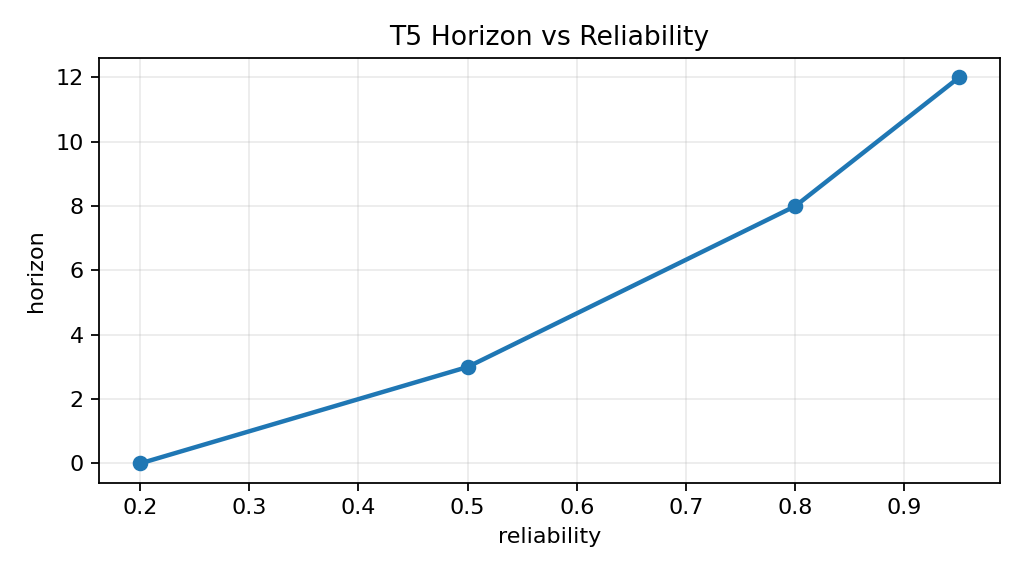
\includegraphics[width=\linewidth]{reports/publication/fig_T5_horizon_vs_reliability.png}%
}{%
\fbox{\parbox{0.9\linewidth}{Missing T5 horizon figure}}%
}
\scriptsize\textit{T5 certificate horizon versus reliability.}
\end{minipage}\hfill
\begin{minipage}[t]{0.48\textwidth}
\centering
\IfFileExists{reports/publication/fig_T8_safety_useful_work_frontier.png}{%
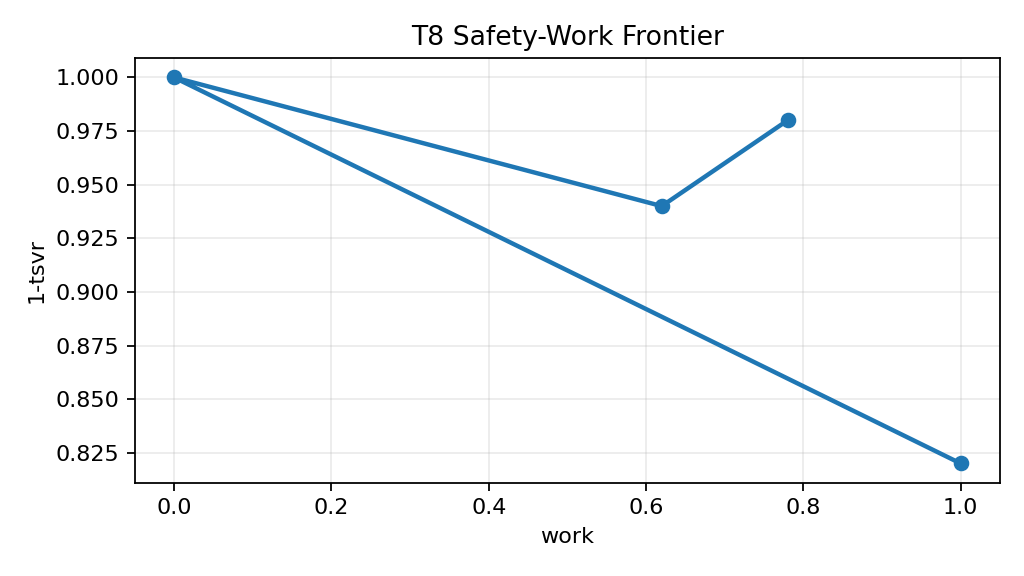
\includegraphics[width=\linewidth]{reports/publication/fig_T8_safety_useful_work_frontier.png}%
}{%
\fbox{\parbox{0.9\linewidth}{Missing T8 useful-work figure}}%
}
\scriptsize\textit{T8 safety--useful-work frontier.}
\end{minipage}
\caption{Temporal-certificate and graceful-degradation theorem artifacts.}
\label{fig:theorem-temporal-graceful-artifacts}
\end{figure}

\begin{figure}[htbp]
\centering
\begin{minipage}[t]{0.48\textwidth}
\centering
\IfFileExists{reports/publication/fig_T10_lower_bound_vs_tv.png}{%
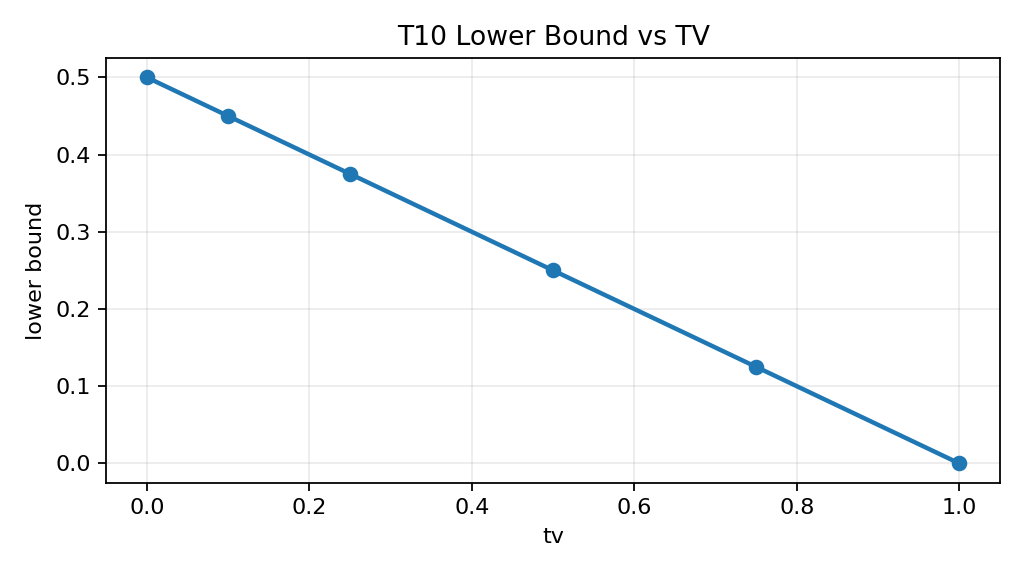
\includegraphics[width=\linewidth]{reports/publication/fig_T10_lower_bound_vs_tv.png}%
}{%
\fbox{\parbox{0.9\linewidth}{Missing T10 lower-bound figure}}%
}
\scriptsize\textit{T10 lower bound versus total variation.}
\end{minipage}\hfill
\begin{minipage}[t]{0.48\textwidth}
\centering
\IfFileExists{reports/publication/fig_Tsensor_safe_core_vs_sensor_drop.png}{%
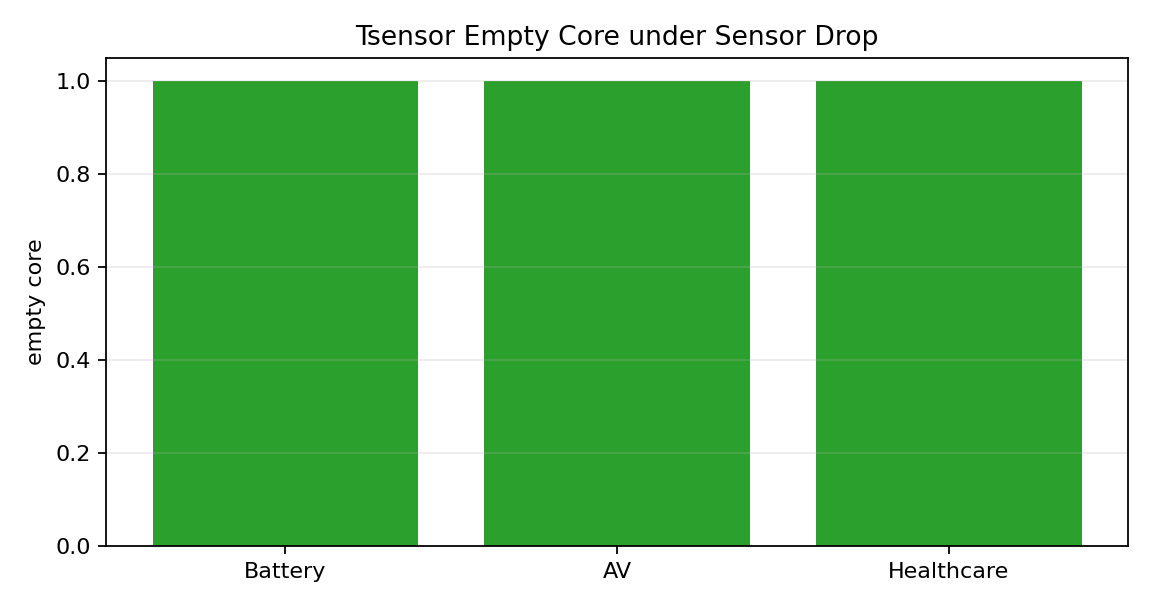
\includegraphics[width=\linewidth]{reports/publication/fig_Tsensor_safe_core_vs_sensor_drop.png}%
}{%
\fbox{\parbox{0.9\linewidth}{Missing sensor-necessity figure}}%
}
\scriptsize\textit{\texttt{T\_sensor\_converse} safe core under sensor ablation.}
\end{minipage}
\caption{Observation-ambiguity lower-bound and sensor-necessity theorem artifacts.}
\label{fig:theorem-ambiguity-sensor-artifacts}
\end{figure}

Appendix~\ref{app:proofs} is the authoritative proof index for the defended
theorem program.  The paper-facing surface intentionally remains narrower: it
inherits the same assumption language and scoped interpretation as the thesis,
but it does not reproduce the full 83-item formal register.

\IfFileExists{paper/assets/tables/generated/tbl_theorem_dependency.tex}{%
% tbl_theorem_dependency.tex
% Theorem dependency and proof completeness (Applied Math Prof critique).
\begin{table}[htbp]
\centering
\caption{DC3S Theorem Dependency and Proof Completeness. Each formal result is implemented in code and tested by at least one automated test.}
\label{tbl:theorem_dependency}
\resizebox{\textwidth}{!}{%
\begin{tabular}{lllll}
\toprule
\textbf{Result} & \textbf{Name} & \textbf{Depends On} & \textbf{Proof Method} & \textbf{Code Reference} \\
\midrule
Defn.~1 & OQE reliability weight $w_t$ & — & Definition & \texttt{quality.py:compute\_reliability()} \\
Prop.~1 & Inflation monotonicity & Defn.~1 & Analytic & \texttt{coverage\_theorem.py:verify\_inflation\_geq\_one()} \\
Thm.~1  & Marginal coverage guarantee & Prop.~1, Defn.~1 & Conformal CP theory & \texttt{coverage\_theorem.py:assert\_coverage\_guarantee()} \\
Thm.~3  & Expected violation bound & Thm.~1 & Expectation calculus & \texttt{coverage\_theorem.py:compute\_expected\_violation\_bound()} \\
Thm.~9  & Group-conditional coverage & Thm.~1 & Mondrian CP & \texttt{coverage\_theorem.py:mondrian\_group\_coverage()} \\
Thm.~10 & Hoeffding high-prob.\ bound & Thm.~3 & Hoeffding inequality & \texttt{coverage\_theorem.py:hoeffding\_violation\_bound()} \\
Thm.~11 & Byzantine OQE reliability bound & Defn.~1 & Trimmed-mean theory & \texttt{quality.py:compute\_reliability\_robust()} \\
\bottomrule
\multicolumn{5}{l}{\small All results are unit-tested in \texttt{tests/test\_conditional\_coverage.py} and \texttt{tests/test\_adversarial\_faults.py}.}\\
\end{tabular}%
}
\end{table}
%
}{%
% tbl_theorem_dependency.tex
% Theorem dependency and proof completeness (Applied Math Prof critique).
\begin{table}[htbp]
\centering
\caption{DC3S Theorem Dependency and Proof Completeness. Each formal result is implemented in code and tested by at least one automated test.}
\label{tbl:theorem_dependency}
\resizebox{\textwidth}{!}{%
\begin{tabular}{lllll}
\toprule
\textbf{Result} & \textbf{Name} & \textbf{Depends On} & \textbf{Proof Method} & \textbf{Code Reference} \\
\midrule
Defn.~1 & OQE reliability weight $w_t$ & — & Definition & \texttt{quality.py:compute\_reliability()} \\
Prop.~1 & Inflation monotonicity & Defn.~1 & Analytic & \texttt{coverage\_theorem.py:verify\_inflation\_geq\_one()} \\
Thm.~1  & Marginal coverage guarantee & Prop.~1, Defn.~1 & Conformal CP theory & \texttt{coverage\_theorem.py:assert\_coverage\_guarantee()} \\
Thm.~3  & Expected violation bound & Thm.~1 & Expectation calculus & \texttt{coverage\_theorem.py:compute\_expected\_violation\_bound()} \\
Thm.~9  & Group-conditional coverage & Thm.~1 & Mondrian CP & \texttt{coverage\_theorem.py:mondrian\_group\_coverage()} \\
Thm.~10 & Hoeffding high-prob.\ bound & Thm.~3 & Hoeffding inequality & \texttt{coverage\_theorem.py:hoeffding\_violation\_bound()} \\
Thm.~11 & Byzantine OQE reliability bound & Defn.~1 & Trimmed-mean theory & \texttt{quality.py:compute\_reliability\_robust()} \\
\bottomrule
\multicolumn{5}{l}{\small All results are unit-tested in \texttt{tests/test\_conditional\_coverage.py} and \texttt{tests/test\_adversarial\_faults.py}.}\\
\end{tabular}%
}
\end{table}
%
}

\section{Risk envelope interpretation}
The risk envelope is the most important bridge between formal and empirical language in the
dissertation. ORIUS does not claim safety from a single forecast error number. It reasons
through miscoverage, intervention feasibility, and mean reliability. That framing is what
allows the theorem layer to connect to uncertainty calibration without collapsing into a
purely statistical dissertation.

In the tightened thesis surface, this bridge is explicit: the episode-level
bound is read through a per-step residual-risk budget, not as a direct
consequence of marginal conformal coverage alone.

The uncertainty references in Chapter~\ref{ch:related-work-novelty-gap} matter here. Classic
conformal prediction supplies the disciplined interpretation of uncertainty sets under
exchangeability, while adaptive conformal methods show how long-run calibration language can
be generalized more honestly under nonstationary streams
\cite{vovk2005algorithmic,romano2019conformalized,gibbs2021adaptive}. ORIUS does not claim
that these methods alone solve runtime safety. It uses them to clarify what the uncertainty
set is allowed to mean before repaired release is evaluated.  In practice, the online
conformal layer is an SPCI-lite quantile tracker in the style of Gibbs and
Candès \cite{gibbs2021adaptive} that maintains an exponentially-weighted sliding window of
conformity scores, yielding intervals that adapt smoothly to distribution shift without a
full recalibration pass.

\section{Why the proofs stay witness-backed but the objects stay universal}
The energy-management reference row remains the deepest theorem-to-code-to-artifact chain because the witness row
provides the richest availability of proof-facing diagnostics, replay traces, and locked
artifacts. That does not make the theorem objects domain-specific. The objects are written
against reliability, uncertainty inflation, admissible action tightening, repair or
fallback, and certificate causality. Those are universal runtime objects instantiated
through the adapter, not energy-management-exclusive definitions.

\section{Theorem-to-artifact linkage}
\begin{figure}[htbp]
\centering
\IfFileExists{reports/publication/fig_integrated_theorem_gate.png}{%
\includegraphics[width=0.88\textwidth]{reports/publication/fig_integrated_theorem_gate.png}%
}{%
\includegraphics[width=0.88\textwidth]{../reports/publication/fig_integrated_theorem_gate.png}%
}
\caption{The integrated theorem gate keeps theorem language aligned to typed contracts,
assumptions, and locked artifacts rather than to informal prose alone.}
\label{fig:integrated-theorem-gate}
\end{figure}

Figure~\ref{fig:integrated-theorem-gate} summarizes the discipline used throughout the
manuscript. Every theorem is attached to an assumption family, a typed runtime object, and
at least one artifact-facing diagnostic or replay surface. This is why the dissertation can
state theorem results without pretending that empirical maturity is equal across all rows.

\section{What is proved, validated, and still open}
The theory chapter therefore ends with an explicit boundary. Theorem statements live here
and in Appendix~\ref{app:proofs}. Validated claims only advance when replay, calibration,
runtime, and governance surfaces exist for the relevant domain row. Roadmap claims remain
outside defended theorem language. That separation is not a stylistic preference. It is the
mechanism that lets ORIUS argue for a universal runtime safety layer without pretending that
broader future-domain empirical closure has already been earned.
